\chapter{Análisis y estudio de los resultados obtenidos}

Una vez expuestas todas las condiciones del entrenamiento, como los modelos a probar, las métricas, funciones de pérdida y presentados los datos, podemos dar paso al entrenamiento. Sin lugar a dudas, es la fase más lenta de todo el proceso, la cual ha prolongado su desarrollo considerablemente. El objetivo es claro: poner a prueba las 5 propuestas realizadas para establecer, en primer lugar, cuál o cuáles de ellas son competitivas, y posteriormente, evaluar todos los conjuntos de datos para medir la ganancia con respecto al conjunto de datos original.

\section{Consideraciones previas: ¿Cómo detectar si un modelo es mejor de manera justa?}

A la hora de realizar las pruebas, existen multitud de factores que pueden influir en los resultados, y los cuales debemos controlar minuciosamente para evitar problemas que alteren los resultados y nos den una idea equivocada del rendimiento. Entre ellos, podemos encontrar las inicializaciones aleatorias de los pesos, el riesgo de sobreaprendizaje y en casos de extremada similaridad de resultados, la calidad semántica aportada por la codificación que estamos evaluando.\\

Para tratar de minimizar el impacto de estos factores y facilitar el análisis de calidad de los positional encodingds propuestos, tomaremos una serie de medidas las cuales examinaremos a continuación.

\subsection{Impacto de la inicialización aleatoria}

Cuando entrenamos cualquier modelo de aprendizaje, en prácticamente cualquier ámbito de problema (datos tabulares, imágenes, secuencias,..) existe un paso el cual muchas veces es ignorado, y que puede afectar considerablemente a los resultados obtenidos: la inicialización de los parámetros del modelo. Aunque este paso podría parecer trivial y de escasa relevancia, debido a que los parámetros serán posteriormente ajustados mediante los mecanismos de aprendizaje, en realidad, puede desempeñar un papel determinante en el rendimiento final del modelo.\\

En la práctica, la inicialización suele realizarse a partir de una distribución pseudoaleatoria generada mediante secuencias controladas por el sistema operativo o el propio lenguaje de programación. Este proceso asigna valores iniciales a cada una de las conexiones y pesos del modelo, y cada valor asignado puede influir considerablemente en la velocidad de convergencia y la estabilidad numérica, ya que los optimizadores que ajustan sus valores posteriormente, se basan en métodos de descenso de gradiente o búsqueda local para tratar de encontrar óptimos locales.\\

Para mejorar la convergencia y eficiencia en entrenamiento, se han desarrollado numerosos optimizadores con el objetivo de evitar quedar atascado durante este proceso y tratar de escapar de óptimos locales de baja calidad que pudieran afectar al resultado final. Uno de los más empleados es Adam~\cite{kingma2017adammethodstochasticoptimization}, el cual utiliza momentum para dotar de cierta inercia a cada una de las dimensiones, ajustando una a una su tasa de aprendizaje, y así tratar de escapar de localidades subóptimas.\\

Por ello, emplearemos este optimizador en el entrenamiento del Transformer, ya que nos permite un enfoque más estable y adaptativo en la actualización de los parámetros y reduciendo la sensibilidad a los pesos y la tasa de aprendizaje inicial.\\
 
Pero esta estrategia no nos exime de los problemas derivados de malas inicializaciones que, de forma fortuita, podrían producir un mal resultado en un modelo que, en condiciones normales, tendría un desempeño superior. Dicho fenómeno puede verse potenciado al emplear los diferentes encodings ponderados, ya que una mala inicialización de alguno de los pesos podría favorecer artificialmente una de las variantes desde el inicio. Aunque el encoding asociado no proporcione un buen rendimiento, la reducción de su valor podría ser lenta, sentenciando el experimento desde el inicio. Para evitarlo, aplicaremos las siguientes soluciones:

\begin{itemize}
	\item Ejecutar todos los experimentos múltiples veces utilizando diferentes semillas aleatorias. Esta práctica nos permitirá reducir el impacto de la aleatoriedad en los modelos, asegurando que los resultados reflejen de manera más fiel el comportamiento real del modelo.
	\item Realizar un inicio uniforme de los pesos de ponderación de encodings. Esto se traduce en establecer como valor de partida a cada peso aprendible un valor equivalente a $1/n$, siendo $n$ el número de alternativas que se desea evaluar. De esta forma, el cálculo empieza sin condiciones de dominancia, y será el propio proceso de aprendizaje el que altere los pesos a su beneficio.
\end{itemize}

 
Gracias a estas soluciones, paliaremos en gran medida el impacto en los resultados. No obstante, debemos tener cuidado con el número de ejecuciones de cada modelo, pues cada una puede requerir varios días de cómputo, lo que nos obliga a buscar un equilibrio entre estabilidad y tiempo. Por lo tanto, excepto si se indica lo contrario, se realizarán tres ejecuciones independientes para cada configuración experimental, calculando posteriormente el promedio estadístico de cada una de las métricas. De esta manera, logramos un \textit{trade-off} adecuado entre ambas condiciones. En conjunto con el uso de Adam, trataremos de maximizar la estabilidad y confiabilidad de los resultados.
 
\subsection{Sobreaprendizaje}

Otro de los problemas destacados durante en el entrenamiento puede ser el sobreaprendizaje. Cuando usamos arquitecturas tan profundas y potentes como los Transformers, es sencillo que la arquitectura tome el conjunto de entrenamiento y lo aprenda de manera bastante próxima a la distribución de estos datos, es decir, la acabe ``memorizando'' y la capacidad de generalización del modelo sea pobre. Esto es especialmente notable en conjuntos de datos más sencillos o de menor longitud, en los que el modelo podría incluso verse algo sobredimensionado. Para evitarlo. se han seleccionado dos estrategias: regularización mediante \textit{dropout} y uso de \textit{early stopping}.

\begin{itemize}
	\item Con el \textbf{early-stopping}, estamos añadiendo un mecanismo de parada automática del entrenamiento, el cual, especificando una paciencia, en épocas, detendremos el modelo en ausencia de mejora. Para controlar esta parada, monitorizaremos el error de pérdida en validación. Para mantener tener una paciencia algo tolerante, escogeremos como valor 3 épocas; si en 3 épocas el error del modelo ha sido peor que el mejor resultado registrado, cancelaremos el proceso, ahorrando recursos de cómputo y evitando mala generalización.
	\item Mediante \textbf{dropout}, evitaremos que la capas totalmente conectadas de la red se sobreespecialicen, desactivando aleatoriamente algunas neuronas en las diferentes iteraciones del entrenamiento. Por defecto, Informer ya incluye un parámetro de dropout, cuyo valor inicial es bastante bajo, 0.05. Este dropout se aplica no solo a las capas del encoder y decoder, sino también a la estructura del embedding de entrada cuando este contiene componentes aprendibles. Dado que ambos elementos presentan comportamientos distintos, y que regularizar los datos de manera excesiva no es conveniente, pues podría perderse información, se ha establecido como criterio aplicar un dropout mayor, de 0.2, para las capas del modelo, mientras que se mantiene el dropout del embedding en su valor original de 0.05. Así, de alguna forma estamos especificando una regla heurística, en la cual mantenemos el índice asociado al embedding 4 veces menor que el aplicado en las capas de la arquitectura.
\end{itemize}

Con el uso de estos dos factores, podremos minimizar el impacto del \textit{overfitting}, y evitar una mala capacidad de generalización del modelo.

\subsection{Comparando la calidad semántica del encoding. Técnica del barajado}

En los aparatados anteriores, hemos destacado constantemente la importancia semántica del positional encoding, y en la importancia de medir adecuadamente la calidad de las codificaciones a través de este aspecto. Sin embargo, la componente semántica es algo completamente externo para una arquitectura de este tipo, ya que las capas de esta solo entienden de valores numéricos y tensores, pero no es capaz de detectar información de significado. Sin embargo, esta puede encontrarse de manera implícita en los datos, en aspectos como la localidad y la detección de patrones, tareas las cuales hemos tratado de modelar en las propuestas de codificación formuladas.\\

Existe una manera muy sencilla de verificar esta propiedad y evaluar la utilidad de la codificación añadida: mezclar la entrada del decoder durante la inferencia y analizar su impacto en la calidad del resultado final, en comparación con una entrada intacta, sin desordenar. Este procedimiento fue propuesto por la publicación \textit{``Are Transformers Effective for Time Series Forecasting?''}~\cite{zeng2022transformerseffectivetimeseries}, y nos permite evidenciar de manera intuitiva la presencia o ausencia de orden y localidad en la codificación.\\

De manera inherente a su estructura, el mecanismo de self-attention de los Transformers es invariante al orden de los elementos de la secuencia. Cuando realizamos el cálculo de las matrices de atención, no estamos realizando más que un producto cruzado de todos los tokens con los demás, por lo que el orden de los productos no afectaría al resultado. Es por ello que se necesita un encoding posicional que permita incluir dicha relación de orden en los datos, y se cumpla esta propiedad esencial necesaria en las series temporales.\\

Sin embargo, en el artículo mencionado se llega a la conclusión de que los mecanismos existentes para los principales modelos del estado del arte, como Informer, Autoformer y FEDformer, con sus respectivas codificaciones temporales, no son capaces de captar el orden natural de los datos. Y va incluso más allá: sustituir todo el mecanismo de atención por una capa totalmente conectada es capaz de ofrecer mejores resultados, y al aplicar el barajado, sí se ve afectada en mayor medida por el desorden. \\

En nuestro caso, teniendo en cuenta que nuestra arquitectura se basa en la estructura de Informer, pero simplificando el mecanismo de atención al prescindir del muestreo y las convoluciones, la escasez mantenimiento del orden podría afectarnos de manera similar. Pero, en este caso, queremos evaluar la efectividad de los métodos de codificación propuestos en este trabajo, por lo que repetiremos el experimento, pero en lugar de hacerlo con la codificación por defecto, que ya conocemos sus resultados, con nuestras alternativas. El objetivo es claro: tratar de demostrar que permiten conservar una mayor semántica de los datos y se ven más perjudicados frente al desorden que la tradicional codificación seno-coseno.

\section{Resultados de los experimentos}

Una vez justificado el procedimiento de ejecución a seguir para los experimentos realizados, podemos comenzar a analizar los resultados obtenidos en el entrenamiento de los mismos. Tal y como se especificó en el capítulo \ref{cap5}, compararemos los resultados haciendo uso de las métricas de regresión especificadas, pero haciendo especial hincapié en el MAE y MSE.\\

La estructura seguida por los experimentos será la siguiente: primero, evaluaremos cuales de las cinco propuestas formuladas obtiene el mejor rendimiento sobre un conjunto de referencia, Household Power Consumption~\cite{hebrail2006individual}, y posteriormente, procederemos a analizar su utilidad en el resto de conjuntos de datos.

\subsection{Evaluación de las alternativas sobre el conjunto HPC}

El dataset de Individual Household Power Consumption ha sido el conjunto escogido para evaluar, en primer lugar, las 5 variantes de nuestro método de encoding. Esta decisión viene motivada por dos aspectos; en primer lugar, este conjunto de datos dispone de una longitud suficiente para inferir la información relevante de la serie y realizar predicciones a largo plazo, y además, en el comportamiento de sus variables vimos aspectos como la estacionalidad, la cual es más difícil de modelar para un Transformer, y ausencia de estacionalidad, lo cual a priori podría suponer un problema para la aplicación de métodos clásicos. Pero, principalmente, la decisión de escoger un dataset viene motivada por le coste computacional: evaluar todas las alternativas en cada uno de los conjuntos de datos podría requerir semanas e incluso meses para completar por cada dataset, lo cual se escapa de los recursos y limitaciones temporales de las que disponemos.\\

\subsubsection{Resultados}

Por lo tanto, escoger un conjunto de datos más manejable como este, de aproximadamente 2 millones de mediciones, y 7 características, supone un interesante campo de pruebas para las codificaciones. Para la comparativa, realizaremos las siguientes ejecuciones:

\begin{itemize}
	\item Informer con configuración por defecto.
	\item PE sinusoidal.
	\item Nuevas propuestas: WinStat, WinStatLag, WinStatFlex,  WinStatTPE y WinStatSPE	
	\item Sin PE.
\end{itemize}

Para realizar una comparativa justa de los resultados, se han empleado en todos los casos los mismos parámetros, de forma que criterios como la longitud de secuencia, la longitud de contexto o la longitud de predicción no afecten a los resultados. La arquitectura y los parámetros asociados se pueden ver en la tabla \ref{ajustes}.

\begin{table}[!ht]
	\centering
	\begin{tabular}{l|l}
		\toprule
		Parámetro & Valor \\
		\midrule
		{Modelo de atención} & Vanilla \\
		{Tamaño de batch} & 32 \\
		{Dropout} & 0.2 \\
		{Nº de ejecuciones} & 3 \\
		{Tamaño de ventana} & 60 \\
		{Longitud de secuencia} & 180 \\
		{Longitud de etiqueta/contexto} & 60 \\
		{Longitud de predicción} & 60 \\
		\bottomrule
	\end{tabular}
\caption{HPC: configuración de parámetros comunes empleada para los experimentos}
\label{ajustes}
\end{table}

\paragraph{Informer}

En primer lugar, comenzaremos por ejecutar el modelo original de Informer. De esta forma, tendremos una referencia de partida que nos sirva para comparar las propuestas siguientes, y ver si están siendo efectivas. Por defecto, Informer usa codificación de tipo seno-coseno, pero adicionalmente, incorpora información de los timestamps a través de un mecanismo llamado timeF. Son características adicionales que tratan de ayudar al modelo a capturar patrones periódicos y estacionales en la serie temporal, aunque de manera bastante limitada. 

\begin{table}[!ht]
	\centering
\begin{tabular}{l|c|c}
	\toprule
	Métrica & Media & STD \\
	\midrule
	MSE & 0,532965 & 0,010976 \\
	MAE & 0,415272 & 0,012216 \\
	MAPE & 2,598725 & 0,066858 \\
	MSPE & 1345,903158 & 113,73071 \\
	RMSE & 0,730005 & 0,00754 \\
	TrainTime(s) & 7817,02026 & 821,270911 \\
	TestTime(s) & 91,941244 & 1.244423 \\
	\bottomrule
\end{tabular}
\caption{HPC: resultados para Informer}
\label{hpcinf}
\end{table}

Los resultados de la ejecución pueden apreciarse en la tabla \ref{hpcinf}. En ella, podemos notar que la varianza en los resultados, tras ejecutar 3 iteraciones, es bastante pequeña, e inferior a la centésima tanto para MAE como MSE. Sin embargo, las tasas de error en las métricas de MAPE y MSPE se disparan: esto se debe a su gran sensibilidad a valores pequeños, ya que todas las mediciones han sido normalizadas, por lo que no deberían ser consideradas como una forma de comparación debida su inestabilidad. En el caso de RMSE, el error también es bastante alto, de un 73\%, fruto de la misma debilidad que la mostrada en MAPE y MSPE.\\

En términos de eficiencia computacional, podemos utilizar el tiempo medio de ejecución como referencia. En promedio, una ejecución del modelo por defecto requiere aproximadamente 7817 segundos, equivalentes a casi 2,17 horas. Aunque este tiempo resulta razonable considerando la longitud del conjunto de datos, su utilidad real es servir como valor de referencia para evaluar el coste adicional que implican las operaciones introducidas en los modelos alternativos que veremos a continuación.

\paragraph{PE sinusoidal}

Continuando con el modelo de referencia, daremos un segundo paso. Teniendo en cuenta el impacto limitado de la información añadida por timeF, ¿es realmente relevante frente a la información proporcionada por el encoding de tipo seno-coseno?. Para conocerlo, hemos realizado una ejecución suprimiendo esta componente, convirtiendo la arquitectura en prácticamente la definición de un Transformer vanilla para procesamiento de lenguaje.\\

Sorprendentemente, los resultados obtenidos, visibles en la tabla \ref{hpcfixed} son muy similares a los vistos en el modelo original: la pérdida de rendimiento en métricas es prácticamente despreciable, con una diferencia de rendimiento inferior a la centésima para el MSE (0,5329 vs 0,5377) y un caso similar en MAE (0,4152 vs 0,414), obteniendo incluso un mejor el resultado para esta codificación. Esto nos indica que la información adicional aportada en el modelo original no estaba aumentando considerablemente el rendimiento del modelo.\\

\begin{table}[!ht]
	\centering
	\begin{tabular}{l|c|c}
		\toprule
		Métrica & Media & STD \\
		\midrule
		MSE & 0,537721 & 0,011375 \\
		MAE & 0,414084 & 0,006756 \\
		MAPE & 2,573043 & 0,094281 \\
		MSPE & 1363,108439 & 117,15614 \\
		RMSE & 0,733254 & 0,007743 \\
		TrainTime(s) & 10741,03553 & 422,837205 \\
		TestTime(s) & 225,145923 & 63,83665 \\
		\bottomrule
	\end{tabular}
	\caption{HPC: resultados para encoding seno-coseno}
	\label{hpcfixed}
\end{table}


Sin embargo, resulta relevante destacar que el tiempo de ejecución aumenta significativamente, alcanzando aproximadamente 10741 segundos (cerca de 3 horas) en el entrenamiento. Aunque este resultado pueda parecer contraintuitivo, ya que eliminar componentes debería reducir el coste, al emplear esta variante el proceso de convergencia del modelo se desarrolla de forma más lenta, y provoca un aumento del tiempo de ejecución. En defintiva, suprimir la información contextual adicional de Informer no empeora gravemente los resultados, pero disminuye la velocidad de convergencia durante el aprendizaje.\\

A continuación, comenzaremos a probar las nuevas alternativas, para ver si consiguen mejorar estos resultados.

\paragraph{WinStat}

Comenzamos por la primera de las propuestas, la cual se basa únicamente en la adición información estadística a través de una ventana deslizante.\\

Recordando su funcionamiento, este método requiere especificar el tamaño de la ventana, la cual recorre los datos para extraer y concatenar información local sobre la media, la desviación estándar y los valores extremos en su entorno. Por tanto, la elección de un tamaño de ventana adecuado resulta crítico para garantizar un rendimiento óptimo, sin comprometer la eficiencia del modelo. Como criterio heurístico, se empleará una longitud comprendida entre un tercio y un cuarto del tamaño de la secuencia de entrada, ya que ofrece un equilibrio razonable entre el mínimo posible, 3, y el extremo opuesto de utilizar una ventana de tamaño longitud de la secuencia.\\

Los resultados para esta alternativa son significativamente mejores y más estables (tabla \ref{hpcwin}) que en los casos anteriores, ya que hemos conseguido reducir tanto MAE como MSE, reduciendo además la varianza de los resultados. Tomando esta última como referencia, podemos apreciar que la mejora es superior a las tres centésimas ($0,502$ vs $0,537$), aportando una mejora considerable del 6\%. Sin embargo, esta mejora de rendimiento ha tenido un gran impacto en el tiempo de cómputo: este es ahora mucho mayor que en casos anteriores, con una variabilidad además mucho más alta, de casi una hora.\\

\begin{table}[!ht]
	\centering
	\begin{tabular}{l|c|c}
		\toprule
		Métrica & Media & STD \\
		\midrule
		MSE & 0,502033 & 0,004632 \\
		MAE & 0,394002 & 0,002849 \\
		MAPE & 2,487715 & 0,090071 \\
		MSPE & 1196,131307 & 105,107660 \\
		RMSE & 0,708535 & 0,003274 \\
		TrainTime(s) & 17697,790107 & 3174,41485 \\
		TestTime(s) & 253,980487 & 3,765932 \\
		\bottomrule
	\end{tabular}
	\caption{HPC: resultados para encoding WinStat}
	\label{hpcwin}
\end{table}

En promedio, se ha requerido $17697$ segundos, unas 4,9 horas, para completar cada ejecución, lo cual es aumento del tiempo de ejecución a prácticamente el doble de Informer original. Si bien la mejora ha sido notable, sería deseable observar si alguna de las siguientes alternativas consigue mejorar la estabilidad numérica y la convergencia de los resultados.

\paragraph{WinStatLags}

WinStatLags es la siguiente propuesta de encoding a evaluar, siguiendo la estrategia especificada de ir aumentando de manera creciente la complejidad de los modelos. La principal característica de este modelo consistía en la incorporación de diferencias mediante lags, las cuales potencian el contexto local. Siguiendo las misma configuración que en los casos anteriores, obtenemos los resultados de la tabla \ref{hpcwinlags}.\\

Volvemos a obtener una mejora pequeña, esta vez del $0,01$ sobre el modelo de ventana sin lags para el MSE, y una reducción del resto de métricas de error, aunque con un empeoramiento marginal registrado en MAE. Aunque dicha diferencia parezca mínima, es significativa si la tenemos en cuenta con respecto al modelo original. Además, en cuestiones de tiempo de ejecución, hemos conseguido unos tiempos de entrenamiento inferiores, sobre todo, gracias a la reducción de la variabilidad de los resultados. Podemos observar que hemos pasado de una varianza cercana a la hora por cada ejecución, a aproximadamente 24 minutos, reduciendo así casi en un tercio la variabilidad del resultado. Esto justifica por tanto la inclusión de esta nueva componente, que se mantiene como estaba previsto en el resto de codificaciones.


\begin{table}[!ht]
	\centering
	\begin{tabular}{l|c|c}
		\toprule
		Métrica & Media & STD \\
		\midrule
		MSE & 0,491026 & 0,004988 \\
		MAE & 0,398612 & 0,005025 \\
		MAPE & 2,312104 & 0,086223 \\
		MSPE & 1012,281759 & 108,01798 \\
		RMSE & 0,700723 & 0,003566 \\
		TrainTime(s) & 13071,568639 & 1403,397188 \\
		TestTime(s) & 229,312370 & 3,086725 \\
		\bottomrule
	\end{tabular}
	\caption{HPC: resultados para encoding WinStatLags}
	\label{hpcwinlags}
\end{table}

\paragraph{WinStatFlex}

WinStatFlex, el siguiente modelo a examinar, combina estadísticos calculados mediante ventanas, diferencias con rezagos anteriores y codificaciones aditivas ponderadas. Su principal ventaja radica en que los pesos de ponderación entrenables, lo que permite una adaptación más precisa al conjunto de datos y ejerce un impacto crítico en el rendimiento final. En este caso, al incorporar PE, LPE y TAPE, junto con la variante basada en ventanas, se dispone de un total de cuatro pesos. Estos fueron inicializados con un valor uniforme de $0,25$, con el fin de evitar problemas de dominancia inicial y garantizar una contribución equilibrada entre componentes.\\

Los resultados de este algoritmo requieren una mayor atención, dada la multitud de resultados que podemos extraer de su rendimiento (ver tabla \ref{hpcflex}):

\begin{table}[!ht]
	\centering
	\begin{tabular}{l|c|c}
		\toprule
		Métrica & Media & STD \\
		\midrule
		MSE & 0,461892 & 0,004841 \\
		MAE & 0,373488 & 0,006858 \\
		MAPE & 2,251120 & 0,091233 \\
		MSPE & 986,080587 & 128,44618 \\
		RMSE & 0,679617 & 0,003558 \\
		TrainTime(s) & 18652,724426 & 128,342962 \\
		TestTime(s) & 350,836037 & 5,567514 \\
		\bottomrule
	\end{tabular}
	\caption{HPC: métricas resultantes para encoding WinStatFlex}
	\label{hpcflex}
\end{table}

\begin{table}[!ht]
	\centering
	\begin{tabular}{l|c}
		\toprule
		Componente & Peso aprendido \\
		\midrule
		Stats & 0,3241 \\
		PE & 0,2355 \\
		LPE & 0,2809 \\
		tAPE & 0,1595 \\
		\bottomrule
	\end{tabular}
	\caption{HPC: valores aprendidos en los pesos del encoding WinStatFlex}
	\label{hpcflexpesos}
\end{table}

\begin{itemize}
	 \item El rendimiento obtenido, tomando como referencia la métrica MSE, es notable. En comparación con el modelo basado en lags y estadísticos, se ha logrado una mejora absoluta de $0,03$, equivalente a un 5,9\%. Este incremento es prácticamente idéntico al observado entre {WinStat} y la codificación original de {Informer}. En términos acumulados, la mejora con respecto a este último alcanza el 13,4\%, lo que representa un avance significativo en el desempeño del modelo. Estos valores demuestran la eficacia de la combinación mediante pesos entrenables.
	\item El tiempo de ejecución, por contra, es el más alto medido hasta el momento, siendo necesario un promedio de 18652 segundos, o 5,2 horas de ejecución, frente a las algo más de 2 horas requeridas por la versión original de Informer. Esta configuración incrementa el tiempo medio de ejecución a más del doble, lo que supone un coste computacional significativamente mayor. No se trata de un enfoque que sobresalga por su rapidez en las fases de entrenamiento e inferencia, pero, sin embargo, la mejora de rendimiento podría convertir esta diferencia en un coste asumible.
	\item El valor final de los pesos (tabla \ref{hpcflexpesos}) tras el entrenamiento nos ofrece información muy valiosa sobre las necesidades de los datos. Las proporciones en promedio alcanzadas por estos indican una mayor inclinación hacia la información semántica de los valores estadísticos, con un 32,41\% de contribución. En el caso de los encodings aditivos, destaca especialmente la componente aprendida por LPE, la cual se adapta lo máximo posible a los datos, y ha adquirido una relevancia del 28,09\%. Tan solo con estas componentes, se cubre una ponderación de 0,605 de los datos, indicando que el modelo tiene una mayor preferencia por aumenta el contexto local de los datos.ç
	
	 El resto de codificaciones presentan valores inferiores, destacando tAPE como la de menor relevancia. Este resultado se explica principalmente por su alta similitud con el resto de codificaciones ponderadas, reduciendo su aporte diferencial dentro del modelo.
	
\end{itemize}

En resumen, este modelo supone un salto considerable frente a todas las alternativas anteriores, y se postula como una de las mejores variantes de las codificaciones propuestas.

\paragraph{WinStatTPE}

Una vez estudiado el excelente rendimiento de WinStatFlex, es el turno de su variante cercana WinStatTPE, la cual sustituye el uso de tAPE por T-PE, que dispone de mayor riqueza semántica, manteniendo una base geométrica tradicional. El funcionamiento se basa en los mismos principios, por lo que pasaremos directamente a los resultados (\ref{hpctpe}):
\begin{table}[!ht]
	\centering
	\begin{tabular}{l|c|c}
		\toprule
		Métrica & Media & STD \\
		\midrule
		MSE & 0,463651 & 0,001917 \\
		MAE & 0,374392 & 0,004132 \\
		MAPE & 2,252478 & 0,001750 \\
		MSPE & 954,171082 & 38,396774 \\
		RMSE & 0,680918 & 0,001408 \\
		TrainTime(s) & 18913,633506 & 28,792701 \\
		TestTime(s) & 296,252991 & 1,955109 \\
		\bottomrule
	\end{tabular}
	\caption{HPC: métricas resultantes para encoding WinStatTPE}
	\label{hpctpe}
\end{table}

\begin{table}[!ht]
	\centering
	\begin{tabular}{l|c}
		\toprule
		Componente & Peso aprendido \\
		\midrule
		Stats & 0,24 \\
		PE & 0,258 \\
		LPE & 0,271 \\
		TPE & 0,231 \\
		\bottomrule
	\end{tabular}
	\caption{HPC: valores aprendidos en los pesos del encoding WinStatTPE}
	\label{hpctpepesos}
\end{table}

\begin{itemize}
	\item Las métricas de rendimiento muestran un resultado bastante similar al modelo proporcionado por la variante Flex, aunque marginalmente peores a este. 
	
	Sin embargo, la varianza de los resultados obtenidos es notablemente menor, denotando una mayor estabilidad numérica, y un posible potencial de generalización más consistente al aplicarse a nuevos datos. Aunque sigue superando a la codificación vanilla de \textit{Informer}, las métricas no muestran diferencias significativas frente a WinStatFlex. No obstante, esta estabilidad podría convertirla en una opción atractiva en contextos distintos, con conjuntos de datos diferentes.
	
	\item El tiempo de ejecución vuelve a ser el principal lastre de la propuesta, siendo, en este caso, aún mayor que la codificación anterior, convirtiéndose en el peor tiempo de ejecución visto hasta el momento, llegando a las 5 horas y cuarto.
	
	\item Los pesos obtenidos al final del aprendizaje, visibles en la tabla \ref{hpctpepesos}, reflejan un ajuste bastante equiparado entre las diferentes componentes del modelo. En este caso, el lugar anteriormente ocupado por tAPE logra remontar su peso hasta el 23,1\%, restando algo de relevancia al peso asociado a la componente estadística, que desciende hasta el 24\%. El resto de componentes permanece similar, pero ahora, la colaboración de las diferentes partes es bastante más equilibrada.
\end{itemize}

En definitiva, este modelo presenta grandes ventajas frente a las codificaciones tradicionales, pero en comparación a la propuesta realizada por WinStatFlex, la diferencia en métricas es marginal, y el coste es superior. Su principal característica parece ser su gran estabilidad numérica, por lo que se mantiene como una alternativa atractiva junto a WinStatFlex.

\paragraph{WinStatSPE}

WinStatSPE será nuestra última variante a probar de las propuestas por este trabajo, y se centrará en evaluar el funcionamiento de un modelo ponderado donde interviene un mecanismo de modificación de atención explícito como es SPE. Las expectativas de rendimiento son bastante bajas, ya que en su definición se destacó su fortaleza en problemas de clasificación, y no mencionan conclusiones acerca de sus resultados en forecasting. Pero debido, a que no se estipularon restricciones acerca de una posible aplicación de un problema de predicción como este, consideramos relevante probar su comportamiento. Por tanto, tomando como codificación posicional estándar la empleada en WinStatFlex, se ha combinado con un modelo alternativo que modifica la atención para incluir SPE. Los resultados obtenidos se pueden ver en la tabla \ref{hpcspe}:
\begin{table}[!ht]
	\centering
	\begin{tabular}{l|c|c}
		\toprule
		Métrica & Media & STD \\
		\midrule
		MAE & 0,441418 & 0,032406 \\
		MAPE & 2,558296 & 0,121722 \\
		MSE & 0,582600 & 0,044727 \\
		MSPE & 1388,203491 & 147,022305 \\
		RMSE & 0,762703 & 0,029725 \\
		TestTime(s) & 1730,330627 & - \\
		TrainTime(s) & 131450,338871 & - \\
		\bottomrule
	\end{tabular}
	\caption{HPC: métricas de rendimiento para WinStatSPE}
\label{hpcspe}
\end{table}


\begin{table}[!ht]
	\centering
	\begin{tabular}{l|c}
		\toprule
		Componente & Peso aprendido \\
		\midrule
		Stats &0,2505 \\
		PE & 0,2361 \\
		LPE &  0,1948 \\
		tAPE &  0,3186 \\
		\bottomrule
	\end{tabular}
	\caption{HPC: valores aprendidos en los pesos del encoding WinStatSPE}
	\label{hpcspepesos}
\end{table}

\begin{itemize}
	\item Las métricas proporcionadas por el modelo contienen peores resultados que el modelo de referencia. Esto indica que evidentemente, algo no esta funcionando adecuadamente a la hora de modificar la atención, ya que de por sí sola, la codificación complementaria que se ha utilizado sí que ofrece buenos resultados. Esto confirma las intuiciones anteriores, y muestra que posiblemente SPE sea efectivamente un método propio de clasificación.
	
	\item El tiempo de ejecución es muy alto en comparación con todos los métodos vistos. Debido a un problema de desbordamiento con las variables de tiempo, no se dispone de varianza, pero teniendo en cuenta el tiempo total y realizando el promedio, se estima que cada iteración de las realizadas duró una media de $131450$ segundos, lo cual equivale aproximadamente a un día y medio (36 horas). Esto pone en evidencia la ineficacia del método tanto a nivel de resultados como computacionalmente. 
	
	El resultado es sorprendente, dado que la definición original de este método lo proponía como una aproximación de la atención completa mediante una distribución normal. Sin embargo, debido probablemente a limitaciones de memoria o de capacidad de cómputo de la CPU, esta alternativa ha mostrado ser más lenta que el cálculo directo de la atención completa. Incluso el tiempo de inferencia ha crecido rozando un rendimiento casi 20 veces más lento.
	
	\item En este caso, los pesos obtenidos presentan un comportamiento inusual (tabla \ref{hpcspepesos}), probablemente debido a la alteración del mecanismo de atención. Se observa una mayor potenciación de la componente tAPE, anteriormente inferior, alcanzando una contribución del 31,86\%, y reduciendo la relevancia de los datos en sí hasta el 25,05\%. 
	
\end{itemize}

En resumen, queda en evidencia que esta modificación, empleando SPE como variante de atención, no aporta resultados positivos. Incluso ejecuta empleando los mecanismos de PE propios de Informer, a modo de descarte, su rendimiento deja mucho que desear, con un MSE de  0,553648. Por tanto, queda eliminado de nuestro conjunto de alternativas de ensayo para los siguientes datasets evaluados.

\paragraph{Informer sin PE}

Una pregunta especialmente relevante, tras todo el proceso visto hasta el momento, es la siguiente: ¿realmente resulta significativo el uso de positional encoding para la predicción de series temporales?\\

La teoría indica que sí, dado que los datos de entrada por sí solos no contienen información explícita sobre el orden temporal, y el cálculo de atenciones, al basarse en productos de matrices, no puede inferirlo por sí solo.  No obstante, para confirmarlo empíricamente, procederemos a evaluar esta alternativa mediante experimentación, y así reafirmar esta idea.

\begin{table}[!ht]
	\centering
	\begin{tabular}{l|c|c}
		\toprule
		Métrica & Media & STD \\
		\midrule
		MSE & 0,544844 & 0,005447 \\
		MAE & 0,421343 & 0,005856 \\
		MAPE & 2,394682 & 0,055825 \\
		MSPE & 1053,862630 & 84,204210 \\
		RMSE & 0,738126 & 0,003690 \\
		TrainTime(s) & 10382,266527 & 2083,316310 \\
		TestTime(s) & 125,053827 & 2,833062 \\
		\bottomrule
	\end{tabular}
	\caption{HPC: métricas de rendimiento para Informer sin PE}
	\label{hpcnope}
\end{table}

En la Tabla \ref{hpcnope} se presentan los resultados del experimento. Tal y como se esperaba, el rendimiento sin positional encoding es inferior al de las codificaciones propuestas, a excepción de SPE, que claramente no correspondía a este ámbito de problemas.\\

Sin embargo, la diferencia con respecto a la arquitectura Informer original es mínima: el rendimiento es muy cercano, con valores de $0.532965$ frente a $0.544844$. Esto indica que la información posicional aportada por el positional encoding en este caso es limitada, ya que el empeoramiento relativo es prácticamente despreciable. Esta observación refuerza aún más la relevancia del trabajo realizado en la optimización y comparación de distintas codificaciones que se viene realizando hasta el momento.

\subsubsection{Elección del mejor modelo}

Tras la ejecución de los ocho experimentos anteriores, hemos obtenido resultados valiosos que nos permiten comparar el rendimiento de todas las codificaciones analizadas. Debido a que las tablas pueden ser algo densas, con el objetivo de visualizar de forma más intuitiva estas diferencias, se ha elaborado un gráfico (figura \ref{hpcgraph}) que resume las métricas principales de cada modelo, MAE y MSE, permitiendo observar de un vistazo el ranking de alternativas ordenadas por MSE.\\

\begin{figure}[!ht]
	\centering
	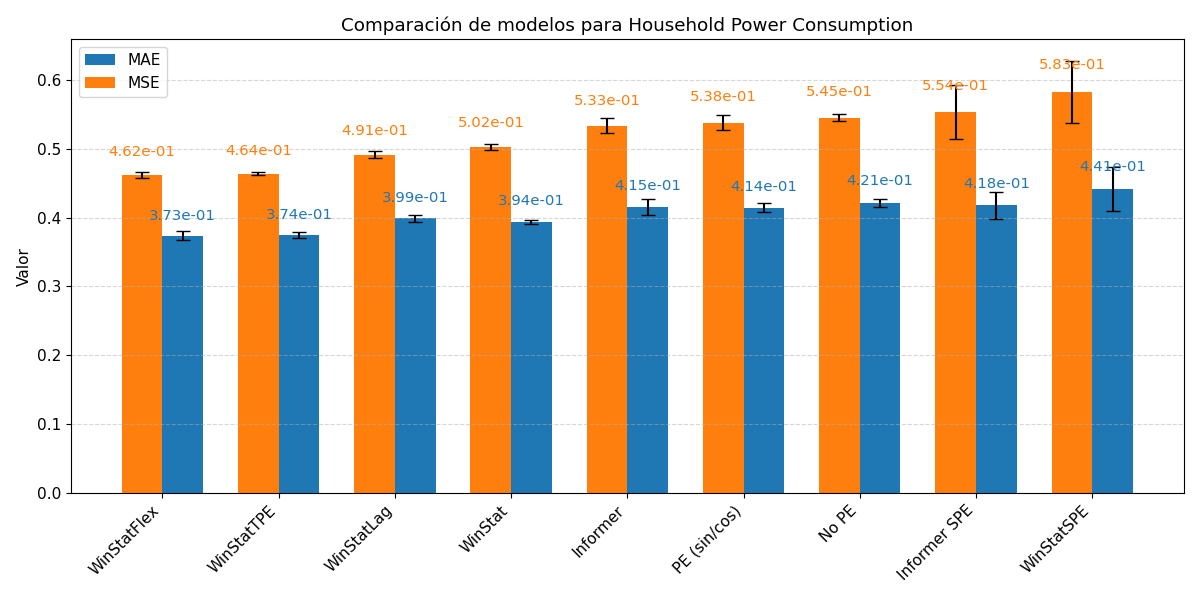
\includegraphics[scale=0.475]{img/hpcgraph}
	\caption{HPC: comparativa gráfica de los positional encodings evaluados}
	\label{hpcgraph}
\end{figure}

En ella, se puede apreciar rápidamente como WinStatFlex y WinStatTPE obtienen el mejor resultado, siendo la variabilidad de T-PE inferior, tal y como indican las barras de error dibujadas.  Informer se sitúa en la parte intermedia de la gráfica, siendo empeorados sus resultados al emplear la codifación fija seno/coseno, no usar codificación, o bien, emplear SPE, el cual ya desestimamos.\\

Si bien todos los modelos propuestos (a excepción de SPE) obtienen mejores resultados frente a Informer, debemos reducir el conjunto de métodos a un número razonable para poder llevar a cabo un experimento similar sobre conjuntos como TINA, de mayor extensión, evitando perder recursos de cómputo en otros PE menos prometedores. Por este motivo, se toma la decisión de continuar únicamente con las alternativas WinStatFlex y WinStatTPE, las cuales han mostrado un buen desempeño en las pruebas realizadas, y ofrecen resultados demasiado cercanos como para discriminar únicamente usando los valores de este conjunto de datos.\\

Y ahora, debemos volver a hacer hincapié sobre el objetivo que estamos persiguiendo: verificar si los nuevos encodings añaden de verdad información semántica. Para ello, realizaremos el experimento anteriormente mencionado del barajado del decoder. Volveremos a ejecutar los dos mejores algoritmos seleccionados e Informer, y ver si realmente se repite la problemática vista en \cite{zeng2022transformerseffectivetimeseries}.\\

En la tabla \ref{hpcresultados_modelos}, podemos encontrar los resultados, del cual podemos extraer varias conclusiones:
\begin{table}[ht]
	\centering
	\begin{tabular}{l|c|c|c|c}
		\toprule
		Modelo & {MAE} & {MAE (STD)} & {MSE} & {MSE (STD)}  \\
		\midrule
		WinStatFlex & 0,373488 & 0,006858 & 0,461892 & 0,004841 \\
		WinStatTPE & 0,374392 & 0,004132 & 0,463651 & 0,001917 \\
		Informer & 0,415272 & 0,012216 & 0,532965 & 0,010976 \\
		No PE & 0,421343 & 0,005856 & 0,544844 & 0,005447 \\
		Informer (Shuffled) & 0,419960 & 0,002769 & 0,548443 & 0,009148 \\
		WinStatFlex (Shuffled) & 0,581124 & 0,021991 & 0,782092 & 0,027368 \\
		WinStatTPE (Shuffled) & 0,581001 & 0,046717 & 0,851115 & 0,024083 \\
		\bottomrule
	\end{tabular}
	\caption{HPC: resultados para experimento de mezcla en encoder}
	\label{hpcresultados_modelos}
\end{table}


\begin{table}[ht]
	\centering
	\begin{tabular}{l|c|c|l|c}
		\toprule
		Modelo & {Tº Test(s)} & {Tº Test(s)-STD} & {Tº Train(s)} & {Tº Train(s)-STD} \\
		\midrule
		WinStatFlex & 350,8360 & 5,5675 & 18652,7244 & 128,3429 \\
		WinStatTPE & 296,2529 & 1,9551 & 18913,6335 & 28,7927 \\
		Informer & 91,9412 & 1,2444 & 7817,0202 & 821,2709 \\
		No PE & 125,0538 & 2,8330 & 10382,2665 & 2083,3163 \\
		Informer (Shuffled) & 85,9877 & 0,7681 & 7923,0834 & 1508,2765 \\
		WinStatFlex (Shuffled) & 330,9885 & 6,0409 & 20842,9511 & 1877,7778 \\
		WinStatTPE (Shuffled) & 295,0051 & 1,2049 & 20580,5136 & 2278,5627 \\
		\bottomrule
	\end{tabular}
	\caption{HPC: Tiempos de ejecución para cada modelo tras el mezclado}
	\label{hpc_tiempos_modelos}
\end{table}

\begin{itemize}
	\item En primer lugar, el rendimiento de Informer original y mezclados es muy similar, con una diferencia mínima entre ellos, respaldando así los resultados realizados en el paper original. La versión sin PE se sitúa justo en medio de ambos resultados, haciendo que los 3 modelos ofrezcan de manera general el mismo rendimiento y afianzando la pobre semántica y mantenimiento de orden que aporta la estrategia tradicional.
	\item WinStatFlex sufre de manera marcada el impacto de aplicar el barajado, lo cual son muy buenos resultados. Esto nos indica que la información aportada por este método es capaz de modelar de manera adecuada tanto el contexto como la estructura inherente de la serie, y que cuando se aplica sobre una entrada mezclada, se produce una gran alteración y degradación del rendimiento. Este comportamiento resulta coherente y lógico desde un punto de vista teórico, y sus efectos se aprecian a nivel empírico: el MSE pasa de $0,461892$ a $0,782092$, lo que supone un empeoramiento relativo del 69,3\%.
	\item WinStatTPE muestra un efecto similar; al aplicar el barajado, pasamos de $0,463651$ a $0,851115$, sufriendo incluso un mayor empeoramiento que la variante Flex. En valores relativos, la diferencia es de un 83,5\%, indicando por tanto que la información semántica aportada por T-PE es aún más sensible a barajado que el resto de codificaciones.
\end{itemize}

Estos resultados refuerzan, por tanto, un mejor aprovechamiento del contexto local y semántico de los datos, siendo ahora una parte clave del modelo que se ve tremendamente afectada cuando realizamos alteraciones que manipulen la estructura y rompan el contexto temporal. Gracias a este experimento, hemos podido verificarlo de manera sencilla y poner en valor los resultados obtenidos. Los tiempos de ejecución han crecido, como era de esperar, en los modelos mezclados (representados como variantes \textit{Shuffled} en la tabla \ref{hpc_tiempos_modelos}), pero dicho sobrecoste asociado es asumible dada la utilidad del procedimiento.\\

\begin{figure}[!ht]
	\centering
	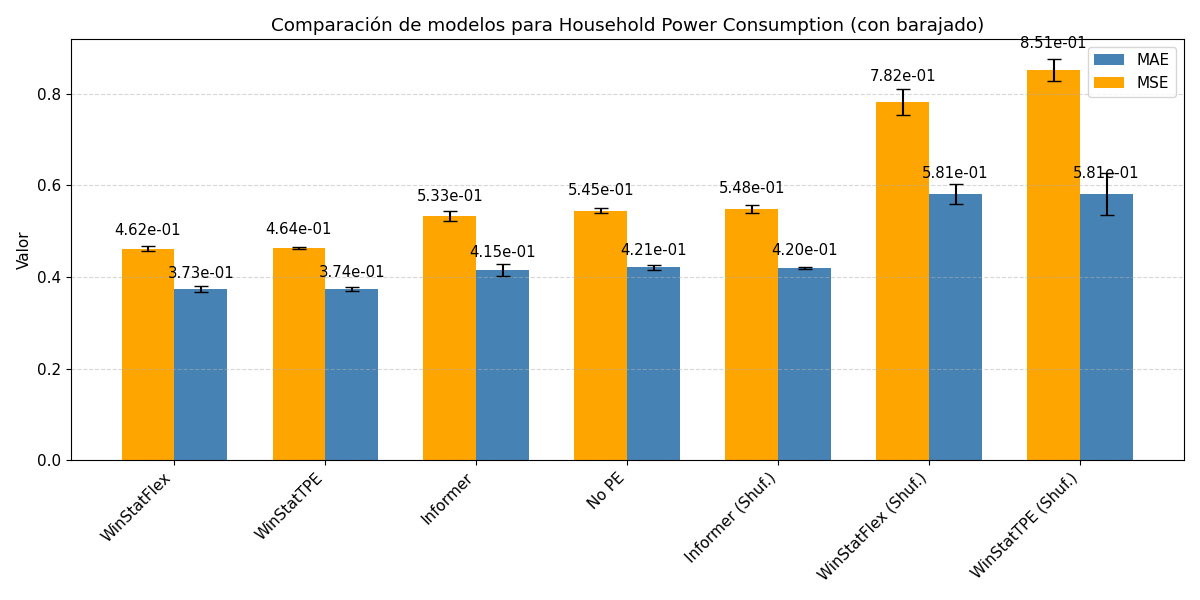
\includegraphics[scale=0.475]{img/hpcgraphshuffled}
	\caption{HPC: comparativa gráfica de los PE, tras aplicar barajado}
	\label{hpcgraphshuffled}
\end{figure}

A modo de resumen final, en la figura \ref{hpcgraphshuffled} se representan los resultados de los modelos comparados con el barajado, para apreciar de manera visual que las diferencias entre pares de modelos ahora son bastante notables en comparación con Informer original.